\section{Formal languages}

\index{natural language}
\index{language!natural}

Learning a programming language is very different from learning a {\bf natural language} such as English, Spanish, or German.
The languages that people speak evolved naturally over time.
%They were not designed by people, although we try to impose order on them for practical reasons.

\index{formal language}
\index{language!formal}

In contrast, {\bf formal languages} are designed by people for specific applications.
For example, the notation that mathematicians use is a formal language that is particularly good at denoting relationships among numbers and symbols.
Chemists use a formal language to represent the chemical structure of molecules.
And most importantly:

\index{programming language}
\index{language!programming}

\begin{quote}
{\bf Programming languages are formal languages that have been designed to express computations.}
\end{quote}

\index{syntax}
\index{semantics}

Formal languages have strict rules about both the {\bf syntax} (structure) and the {\bf semantics} (meaning) of statements.
For example, $3 + 3 = 6$ is a syntactically correct mathematical statement, but $3\ + = 3\ \$\ 6$ is not.
$1 + 2 = 4$ uses correct syntax, but is semantically incorrect.
$H_2O$ is a syntactically correct chemical formula, but $_2Zz$ is not.

%\subsection{Tokens and grammar}

\index{token}

Syntax rules come in two flavors, pertaining to tokens and grammar.
{\bf Tokens} are the basic elements of the language, like words, numbers, and chemical elements.
One of the problems with $3\ + = 3\ \$\ 6$ is that $\$$ is not a legal token in mathematics.
Similarly, $_2Zz$ is not legal because there is no element with the abbreviation $Zz$.

\index{grammar}

The second type of syntax rule pertains to the {\bf grammar} of the language, or the way tokens can be arranged.
The statement $3\ + = 3$ is structurally illegal, even though $+$ and $=$ are legal tokens, because you can't have one right after the other.
Similarly, in a chemical formula the subscript comes after the element name, not before.

\index{parse}

When you read a sentence in English or a statement in a formal language, you have to figure out its structure.
This process is called {\bf parsing}, and in a natural language you learn to do it unconsciously.
As you learn to program, you will learn to parse Java code.

%For example, when you hear the statement ``the penny dropped,'' you understand that the penny is the subject and ``dropped'' is the predicate.
%After you have parsed the statement, you can begin to figure out what it means.
%Assuming that you know what a penny is and what it means to drop, you will understand the general implication of this statement.

%\subsection{Reading source code}

Beginning programmers, who are used to natural languages, often have a hard time adjusting to formal languages.
Although formal and natural languages have features in common---tokens, grammar, and meaning---there are some differences:

\begin{description}

\term{ambiguity}
Natural languages are full of ambiguity, which people deal with by using contextual clues and other information.
Formal languages are designed to be nearly or completely unambiguous, which means that any statement has exactly one meaning, regardless of context.

\term{redundancy}
In order to make up for ambiguity and reduce misunderstandings, natural languages employ lots of redundancy.
As a result, they are often verbose.
Formal languages are less redundant and more concise.

\term{literalness}
Natural languages are full of idiom and metaphor.
When someone says ``the penny dropped'' there is no penny and nothing dropping.
This idiom means that someone finally realized something after a period of confusion.
In contrast, formal languages mean exactly what they say.

\end{description}

%In some ways, the difference between natural and formal language is like the difference between poetry and prose, but more so.

%\begin{description}

%\term{poetry}
%Words are used for their sounds as well as for their meaning, and the whole poem together creates an effect or emotional response.
%Ambiguity is not only common but often deliberate.

%\term{prose}
%The literal meaning of words is more important, and the structure contributes more meaning.
%Prose is more amenable to analysis than poetry but still often ambiguous.

%\term{program}
%The meaning of a computer program is unambiguous and literal, and can be understood entirely by analysis of the tokens and grammar.

%\end{description}

%Here are some suggestions for reading programs (and other formal languages).

Small errors in spelling and punctuation, which you can get away with in natural languages, can make a big difference in a formal language.

Also, formal languages are more dense than natural languages, so it takes longer to read them.
The structure is very important, so it is not always a good idea to read from top to bottom, left to right.
Over time you will learn to parse programs in your head, identifying the tokens and interpreting the structure.
And you will learn to read and write programs more quickly.


%\term{natural language}
%Any of the languages people speak that have evolved naturally.

%\term{formal language}
%A language people have designed for specific purposes, like representing mathematical ideas or computer programs.

%\term{programming language}
%A formal language that has been designed to express computations.

%\term{syntax}
%The structure of a program.

%\term{semantics}
%The meaning of a program.

%\term{token}
%A basic element of a program, such as a word, space, symbol, or number.

%\term{grammar}
%A set of rules that determines whether a statement is legal.

%\term{parse}
%To examine a program and analyze the syntactic structure.


\section{Syntax errors}

\index{syntax error}
\index{error!syntax}

{\bf Syntax} pertains to the structure of a program and the arrangement of the words and symbols it contains.
Programming languages have syntax rules.
For example, parentheses have to come in matching pairs.
So \java{(1 + 2)} is legal, but \java{8)} is not.
If you violate a syntax rule, you have committed a {\bf syntax error}.
In that case, you program cannot be translated or run; instead, the compiler stops and displays an error message.

\begin{figure}[!h]
\begin{center}
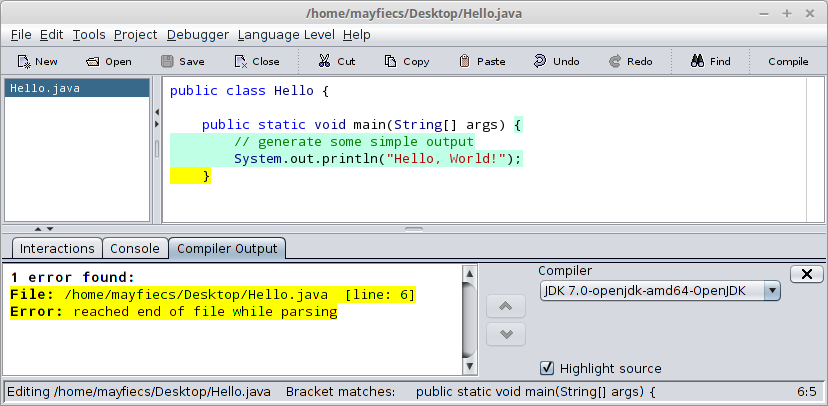
\includegraphics[width=\textwidth]{figs/syntax-error.png}
\caption{A syntax error caused by a missing brace.}
\label{fig:syntax}
\end{center}
\end{figure}

As shown in Figure~\ref{fig:syntax}, removing the closing brace on line 8 of the hello world program results in ``Error: reached end of file while parsing.''
The compiler also reports that the problem was found on line 6, which in this case is not at fault.
Since line 8 was deleted, the compiler reported the last line of the file.


\section{Type conversion}

%The difference is when the conversion from integer to string actually takes place.

%Fortunately, this situation only happens when using the plus operator.
%You cannot, for example, store an integer directly in a string variable.
%
%\begin{code}
%     String number = 5;  // syntax error
%\end{code}

%In general, it's better not to compose multiple additions of varying data types.
%Instead you can break those statements into multiple lines, or use another method like \java{printf} to achieve the same results.

% TODO: add the following subsection before/after operators for strings?
% ABD: maybe not: we have an exercise about this

%\index{type!conversion}
%\index{typecasting}

%You might wonder how you can get away with an expression like \java{
%"The log of x is " + result}, since one of the operands is a \java{String}
%and the other is a \java{double}.  In this case Java is being
%smart on our behalf, automatically converting the \java{double} to a
%\java{String} before it does the string concatenation.

%This kind of feature is an example of a common problem in designing a
%programming language, which is that there is a conflict between {\em
%formalism}, which is the requirement that formal languages should have
%simple rules with few exceptions, and {\em convenience}, which is the
%requirement that programming languages be easy to use in practice.

%More often than not, convenience wins, which is usually good for
%expert programmers (who are spared from rigorous but unwieldy
%formalism), but bad for beginning programmers, who are often baffled
%by the complexity of the rules and the number of exceptions.  In this
%book I have tried to simplify things by emphasizing the rules and
%omitting many of the exceptions.

%Whenever you try to ``add'' two
%expressions, if one of them is a \java{String}, Java converts the
%other to a \java{String} and then performs string concatenation.
%What do you think happens if you perform an operation between
%an integer and a floating-point value?


\section{Increment and decrement}

\index{operator!increment}
\index{operator!decrement}

Incrementing and decrementing are such common operations that Java provides special operators for them.
The {\tt ++} operator adds one to the current value of an {\tt int} or {\tt char}.
{\tt --} subtracts one.
Neither operator works on {\tt double}s, {\tt boolean}s or {\tt String}s.

Technically, it is legal to increment a variable and use it in an expression at the same time.
For example, you might see something like:

\begin{code}
    System.out.println(i++);
\end{code}

Looking at this, it is not clear whether the increment will take effect before or after the value is printed.
Because expressions like this tend to be confusing, I discourage you from using them.
In fact, to discourage you even more, I'm not going to tell you what the result is.
If you really want to know, you can try it.

Using the increment operators, we can rewrite the letter-counter:

\begin{code}
    int index = 0;
    while (index < length) {
        if (fruit.charAt(index) == 'a') {
            count++;
        }
        index++;
    }
\end{code}

It is a common error to write something like

\begin{code}
    index = index++;             // WRONG!!
\end{code}

Unfortunately, this is syntactically legal, so the compiler will not warn you.
The effect of this statement is to leave the value of {\tt index} unchanged.
This is often a difficult bug to track down.

Remember, you can write {\tt index = index+1}, or you can write {\tt index++}, but you shouldn't mix them.


\section{Class definitions and object types}

Here are some syntax issues about class definitions:

\begin{itemize}

\item Class names (and hence object types) should begin with a capital letter, which helps distinguish them from primitive types and variable names.

\item You usually put one class definition in each file, and the name of the file must be the same as the name of the class, with the suffix {\tt .java}.
For example, the \java {class Time} is defined in the file named {\tt Time.java}.

\item In any program, one class is designated as the {\bf startup class} that contains a method named \java{main} where the execution of the program begins.
Other classes {\em may} have a method named \java{main}, but it will not be executed (unless another method calls it directly for some reason).

\end{itemize}

\term{startup class}
The class that contains the \java{main} method where execution of the program begins.

\term{pure function}
A method whose result depends only on its parameters, and that has no side-effects other than returning a value.


\section{Objects and primitives}

\index{type!object}
\index{type!primitive}
\index{object type}
\index{primitive type}

There are two kinds of types in Java, primitive types and reference types.
Primitives, like \java{int} and \java{char} begin with lowercase letters; reference types like \java{String} begin with uppercase letters.
This distinction is useful because it reminds us of some of the differences between them:

\begin{itemize}

\item When you declare a primitive variable, you get storage space for a primitive value.
When you declare a reference variable, you only get space for a reference to an object.
To get space for the object itself, you have to use \java{new}.

\item If you don't initialize a primitive type, it is given a default value that depends on the type.
For example, {\tt 0} for {\tt int}s and {\tt false} for {\tt boolean}s.
The default value for object types is {\tt null}, which indicates no object.

\item Primitive variables are well isolated in the sense that there is nothing you can do in one method that will affect a variable in another method.
Object variables can be tricky to work with because they are not as well isolated.
If you pass a reference to an object as an argument, the method you invoke might modify the object, in which case you will see the effect.
Of course, that can be a good thing, but you have to be aware of it.

\end{itemize}

There is one other difference between primitives and object types.
You cannot add new primitives to Java (unless you get yourself on the standards committee), but you can create new object types!  We'll see how in the next chapter.


% was in Chapter 8 Strings and Things
\begin{exercise}
If you did the GridWorld exercises in Chapter~\ref{gridworld1}, you
might enjoy this exercise.  The goal is to use trigonometry to get the
Bugs to chase each other.

Make a copy of {\tt BugRunner.java} named {\tt ChaseRunner.java} and
import it into your development environment.  Before you change
anything, check that you can compile and run it.

\begin{itemize}

\item Create two Bugs, one red and one blue.

\item Write a method called {\tt distance} that takes two Bugs
and computes the distance between them.  Remember that you can
get the x-coordinate of a Bug like this:

\begin{code}
    int x = bug.getLocation().getCol();
\end{code}

\item Write a method called {\tt turnToward} that takes two
Bugs and turns one to face the other.  HINT: use {\tt Math.atan2},
but remember that the result is in radians, so you have to
convert to degrees.  Also, for Bugs, 0 degress is North, not East.

\item Write a method called {\tt moveToward} that takes two
Bugs, turns the first to face the second, and then moves the
first one, if it can.

\item Write a method called {\tt moveBugs} that takes two Bugs
and an integer {\tt n}, and moves each Bug toward the other {\tt n}
times.  You can write this method recursively, or use a while loop.

\item Test each of your methods as you develop them.  When they are
  all working, look for opportunities to improve them.  For example,
  if you have redundant code in {\tt distance} and {\tt turnToward},
  you could encapsulate the repeated code in a method.

\end{itemize}
\end{exercise}


% was in Chapter 8 Strings and Things
\begin{exercise}
What is the output of the following program?

\begin{code}
public class Enigma {

    public static void enigma(int x) {
        if (x == 0) {
            return;
        } else {
            enigma(x / 2);
        }
        System.out.print(x % 2);
    }

    public static void main(String[] args) {
        enigma(5);
        System.out.println("");
    }
}
\end{code}

Explain in 4-5 words what the method {\tt enigma} really does.
\end{exercise}


\section{Operations on objects}
\label{objectops}
\index{object}
\index{operator!object}

In the next few
sections, I demonstrate three kinds of methods that
operate on objects:

\begin{description}

\item[pure function:]  Takes objects as
arguments but does not modify them.  The return value is
either a primitive or a new object created inside the method.

\item[modifier:]  Takes objects as arguments and modifies some
or all of them.  Often returns void. \index{void}

\item[fill-in method:]  One of the arguments is an ``empty''
object that gets filled in by the method.  Technically, this is
a type of modifier.

\end{description}

Often it is possible to write a given method as a pure function, a modifier,
or a fill-in method.  I will discuss the pros and cons of each.


\section{Fill-in methods}
\index{fill-in method}
\index{method!fill-in}

Instead of creating a new object every time {\tt addTime} is invoked, we could require the caller to provide an object where {\tt addTime} stores the result.
Compare this to the previous version:

\begin{code}
    public static void addTimeFill(Time t1, Time t2, Time sum) {
        sum.hour = t1.hour + t2.hour;
        sum.minute = t1.minute + t2.minute;
        sum.second = t1.second + t2.second;

        if (sum.second >= 60.0) {
            sum.second -= 60.0;
            sum.minute += 1;
        }
        if (sum.minute >= 60) {
            sum.minute -= 60;
            sum.hour += 1;
        }
    }
\end{code}

The result is stored in {\tt sum}, so the return type is {\tt void}.

Modifiers and fill-in methods are efficient because they don't have to create new objects.
But they make it more difficult to isolate parts of a program; in large projects they can cause errors that are hard to find.

Pure functions help manage the complexity of large projects, in part by making certain kinds of errors impossible.
Also, they lend themselves to certain kinds of composition and nesting.
And because the result of a pure function depends only on the parameters, it is possible to speed them up by storing previously-computed results.

\index{pure function}

I recommend that you write pure functions whenever it is reasonable, and resort to modifiers only if there is a compelling advantage.

%\term{fill-in method}
%A type of method that takes an ``empty'' object as a parameter and fills in its instance variables instead of generating a return value.


\section{Incremental development}

\index{incremental development}
\index{prototyping}
\index{program development!incremental}
\index{program development!planning}

In this chapter I demonstrated a program development process called
{\bf rapid prototyping}\footnote{What I am calling rapid prototyping
  is similar to test-driven development (TDD); the difference is that
  TDD is usually based on automated testing.  See
  \url{http://en.wikipedia.org/wiki/Test-driven_development}.}.  For
each method, I wrote a rough draft that performed the
basic calculation, then tested it on a few cases, correcting flaws
as I found them.

This approach can be effective, but it can lead to code
that is unnecessarily complicated---since it deals with many
special cases---and unreliable---since it is hard to convince
yourself that you have found {\em all} the errors.

An alternative is to look for insight
into the problem that can make the programming easier.  In
this case the insight is that a {\tt Time} is really a three-digit
number in base 60!  The {\tt second} is the ``ones column,''
the {\tt minute} is the ``60's column'', and the {\tt hour}
is the ``3600's column.''

When we wrote {\tt addTime} and {\tt increment}, we were effectively
doing addition in base 60, which is why we had to ``carry'' from one
column to the next.

\index{arithmetic!floating-point}

Another approach to the whole problem is to convert
{\tt Time}s into {\tt double}s and take advantage of the fact that
the computer already knows how to do arithmetic with {\tt double}s.
Here is a method that converts a {\tt Time} into a {\tt double}:

\begin{code}
    public static double convertToSeconds(Time t) {
        int minutes = t.hour * 60 + t.minute;
        double seconds = minutes * 60 + t.second;
        return seconds;
    }
\end{code}

Now all we need is a way to convert from a {\tt double}
to a {\tt Time} object.  We could write a method to
do it, but it might make more sense to write it as a third
constructor:

\begin{code}
    public Time(double secs) {
        this.hour =(int)(secs / 3600.0);
        secs -= this.hour * 3600.0;
        this.minute =(int)(secs / 60.0);
        secs -= this.minute * 60;
        this.second = secs;
    }
\end{code}

This constructor is a little different from the others;
it involves some calculation along with assignments to the
instance variables.

You might have to think to convince yourself that the technique
I am using to convert from one base to another is correct.  But once
you're convinced, we can use these methods to rewrite {\tt addTime}:

\begin{code}
    public static Time addTime(Time t1, Time t2) {
        double seconds = convertToSeconds(t1) + convertToSeconds(t2);
        return new Time(seconds);
    }
\end{code}

This is shorter than the original version, and it is much easier
to demonstrate that it is correct (assuming, as usual, that the
methods it invokes are correct).  As an exercise, rewrite {\tt
increment} the same way.


\section{Generalization and algorithms}

\index{generalization}

In some ways converting from base 60 to base 10 and back is
harder than just dealing with times.  Base conversion is more
abstract; our intuition for dealing with times is better.

But if we have the insight to treat times as base 60 numbers,
and make the investment of writing the conversion methods
({\tt convertToSeconds} and the third constructor), we get
a program that is shorter, easier to read and debug, and more
reliable.

It is also easier to add features later.  Imagine
subtracting two {\tt Time}s to find the duration between them.  The
naive approach would be to implement subtraction complete with
``borrowing.''  Using the conversion methods would be much easier.

Ironically, sometimes making a problem harder (more general)
makes it easier (fewer special cases, fewer opportunities for error).

%TODO show solution?

%\section{Algorithms}
%\label{algorithm}

\index{algorithm}

When you write a general solution for a class of problems, as
opposed to a specific solution to a single problem, you have
written an {\bf algorithm}.  This word is
not easy to define, so I will try a couple of approaches.

First, consider some things that are not algorithms.  When you learned
to multiply single-digit numbers, you probably memorized the
multiplication table.  In effect, you memorized 100 specific
solutions, so that knowledge is not really algorithmic.

But if you were ``lazy,'' you probably learned a few
tricks.  For example, to find the product of $n$ and 9, you can
write $n-1$ as the first digit and $10-n$ as the second digit.  This
trick is a general solution for multiplying any single-digit number by 9.
That's an algorithm!

Similarly, the techniques you learned for addition with carrying,
subtraction with borrowing, and long division are all algorithms.  One
of the characteristics of algorithms is that they do not require any
intelligence to carry out.  They are mechanical processes in which
each step follows from the last according to a simple set of rules.

In my opinion, it is embarrassing that humans spend so much
time in school learning to execute algorithms that,
quite literally, require no intelligence.
%
On the other hand, the process of designing algorithms is
interesting, intellectually challenging, and a central part
of what we call programming.

Some of the things that people do naturally, without difficulty
or conscious thought, are the most difficult to express
algorithmically.  Understanding natural language is a good
example.  We all do it, but so far no one has been able to
explain {\em how} we do it, at least not in the form of an
algorithm.

%~ Soon you will have the opportunity to design
%~ simple algorithms for a variety of problems.

%\item[algorithm:]  A set of instructions for solving a class of
%problems by a mechanical process.


\section{Decks and subdecks}
\index{deck}
\index{subdeck}

\index{prototype}
Here is the prototype (see Section~\ref{documentation}) of \java{findBisect}:

\begin{code}
public static int findBisect(Card[] deck, Card card, int low, int high)
\end{code}

\index{parameter!abstract}
\index{abstract parameter}

We can think of \java{cards}, \java{low}, and \java{high} as a single parameter that specifies a {\bf subdeck}.
This way of thinking is common, and is sometimes referred to as an {\bf abstract parameter}.
What I mean by ``abstract'' is something that is not literally part of the program text, but which describes the function of the program at a higher level.

For example, when you invoke a method and pass an array and the bounds \java{low} and \java{high}, there is nothing that prevents the invoked method from accessing parts of the array that are out of bounds.
So you are not literally sending a subset of the deck; you are really sending the whole deck.
But as long as the recipient plays by the rules, it makes sense to think of it abstractly as a subdeck.

This kind of thinking, in which a program takes on meaning beyond what is literally encoded, is an important part of thinking like a computer scientist.
The word ``abstract'' gets used so often and in so many contexts that it comes to lose its meaning.
Nevertheless, {\bf abstraction} is a central idea in computer science (and many other fields).

\index{abstraction}

A more general definition of ``abstraction'' is ``The process of modeling a complex system with a simplified description to suppress unnecessary details while capturing relevant behavior.''

%\term{abstract parameter}
%A set of parameters that act together as a single parameter.

%\term{abstraction}
%The process of interpreting a program (or anything else) at a higher level than what is literally represented by the code.


\section{The Point class}

When you define a class in Java, you are also defining a new data type.
It is helpful to think of classes as the blueprints (or a template) for objects.
To illustrate this point (pun intended), here is a simplified version of the source code for the \java{java.awt.Point} class:

\begin{code}
public class Point {

    public int x;
    public int y;

    public Point(int x, int y) {
        this.x = x;
        this.y = y;
    }

    public String toString() {
        return "Point[x=" + x + ",y=" + y + "]";
    }

}
\end{code}

There are several details to note in this example.

\begin{itemize}

\item The class defines two variables (attributes) named \java{x} and \java{y} that are shared across all methods.
Because they are declared at the class level, their scope is the entire class.

\item The method \java{public Point(int x, int y)} is called a {\bf constructor}.
Its purpose is to initialize new objects, and it is called by the \java{new} operator.
Notice that it has no return type (not even \java{void}).

\item The parameters \java{x} and \java{y} in the constructor happen to have the same name as the attributes.
In order to distinguish one variable from the other, the keyword \java{this} refers to the current object.

%\item None of the variables or methods are \java{static}.
%In other words, they apply to each object of the class as opposed to the class itself.
%We will discuss this issue more deeply in the next chapter.

\end{itemize}

In practice, it's more convenient to look at high-level pictures than source code.
{\bf Unified Modeling Language} (UML) defines a standard way to visualize class designs.
Here is a {\bf class diagram} for the simplified \java{Point} class above:

\begin{center}
\vspace{1ex}
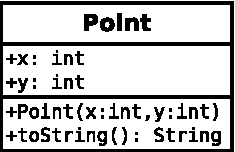
\includegraphics{figs/point.pdf}
\vspace{1ex}
\end{center}

The diagram is divided into two sections: the attributes (or variables) of the class, and the methods of the class.


\index{instance variable}
\index{variable!instance}

The attributes that make up an object are also called instance variables, because each object has its own copy of the variables.
Classes define new data types, and each object is an {\bf instance} of that type.

It's like the glove compartment of a car.
Each car is an instance of the type ``Car,'' and each car has its own glove compartment.
If you ask me to get something from the glove compartment of your car, you have to tell me which car is yours.
